\documentclass[a4j]{jarticle}
\usepackage{ascmac}
\usepackage[dvipdfmx]{graphicx}
\usepackage{listings,jvlisting, jlisting}

\lstset{
  basicstyle={\ttfamily},
  identifierstyle={\small},
  commentstyle={\smallitshape},
  keywordstyle={\small\bfseries},
  ndkeywordstyle={\small},
  stringstyle={\small\ttfamily},
  frame={tb},
  breaklines=true,
  columns=[l]{fullflexible},
  numbers=left,
  xrightmargin=0zw,
  xleftmargin=3zw,
  numberstyle={\scriptsize},
  stepnumber=1,
  numbersep=1zw,
  lineskip=-0.5ex
}

\begin{document}

\vfill
\begin{screen}
  \begin{center}
    \huge\bf 実験　第3回レポート\\
    \vspace{5mm}
    \large\bf
    学籍番号　2022311042 \quad 名前 神野友哉\\
    \today
  \end{center}
\end{screen}
\thispagestyle{empty}

\section{実験}
\subsection{目的}
\vspace{15mm}
\subsection{方法}
\vspace{15mm}
\subsection{結果}
\vspace{15mm}
\subsection{コメント}

\newpage
\section{実験3-1}
実験3-1に用いたラベリング手法の原理を説明し、実験結果が正しい裏付けになる
出力画像\quad G\quad のデータの一部を示せ
\subsection{考察}


\newpage
\begin{figure}[htbp]
  \begin{minipage}{0.5\hsize}
    \begin{center}
      
\includegraphics[width=70mm]{zukei.png}
    \end{center}
    \caption{zukei.pbm}
    \label{fig:z1}
  \end{minipage}
  \begin{minipage}{0.5\hsize}
    \begin{center}
      
\includegraphics[width=70mm]{zukei-label-out.png}
    \end{center}
    \caption{ラベリング後}
    \label{fig:zl}
  \end{minipage}
\end{figure}
\lstinputlisting[caption=rinkaku-label-pbm.c]{rinkaku-label-pbm.c}

\newpage
\section{実験3-2}
実験3-2に用いる特徴計算の方法を説明し、各物体の中心点、周囲長、
面積と複雑度を表で示せ
\subsection{考察}



\newpage
\begin{figure}[htbp]
    \begin{center}
      
\includegraphics[width=100mm]{zukei.png}
    \end{center}
    \caption{zukei.pbm}
    \label{fig:z2}
\end{figure}
\begin{figure}[htbp]
    \begin{center}
      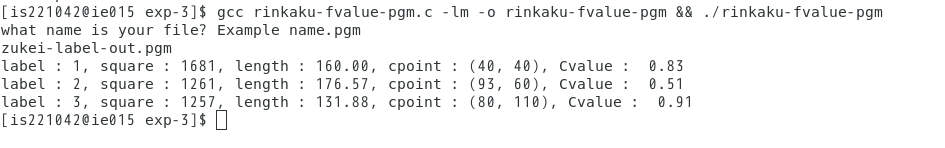
\includegraphics[width=100mm]{fvalue.png}
    \end{center}
    \caption{特徴量}
    \label{fig:fv}
\end{figure}
\lstinputlisting[caption=rinkaku-fvalue-pgm.c]{rinkaku-fvalue-pgm.c}

\newpage
\section{実験3-3}
実験3-3の出力画像Gを示し、特徴計算の具体的な応用について考察せよ
\subsection{考察}



\newpage
\begin{figure}[htbp]
  \begin{minipage}{0.5\hsize}
    \begin{center}
      
\includegraphics[width=70mm]{zukei.png}
    \end{center}
    \caption{zukei.pbm}
    \label{fig:z3}
  \end{minipage}
  \begin{minipage}{0.5\hsize}
    \begin{center}
      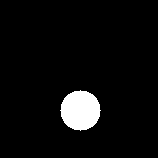
\includegraphics[width=70mm]{zukei-label-out-circle-out.png}
    \end{center}
    \caption{zukei-label-out-circle-out.pgm}
    \label{fig:zlc}
  \end{minipage}
\end{figure}
\lstinputlisting[caption=rinkaku-circle-pgm.c]{rinkaku-circle-pgm.c}

\end{document}
